\documentclass[11pt]{article}
\usepackage[review]{acl}
\usepackage{times}
\usepackage[T1]{fontenc}
\usepackage[utf8]{inputenc}
\usepackage{microtype}
\usepackage{booktabs}
\usepackage{array}
\usepackage{graphicx}
\usepackage{tikz}
\usepackage{pgfplots}
\pgfplotsset{compat=1.18}
\definecolor{armzero}{HTML}{246580}
\definecolor{armfour}{HTML}{BD6338}
\definecolor{armsixteen}{HTML}{707B65}
\usepackage{xurl}
\newcommand{\code}[1]{\texttt{#1}}
\title{Methods of Finding Longer, Readable Palindromes}
\hypersetup{pdftitle={Methods of Finding Longer, Readable Palindromes}}
\hypersetup{pdfsubject={Public release v1}}
\author{Anonymous submission}

\begin{document}
\maketitle

\begin{abstract}
Finding a long palindrome is only part of the problem: it should also make sense. We search for palindromes of 30--119 letters and test a simple idea: discourage phrases that the search keeps reusing. Across 360 matched runs, we compare the original scoring rule with two strengths of this penalty. Each setting returns 90 exact outputs from 120 attempts. Both penalties remove all six targeted phrases and increase distinct outputs from 69 to 78. Yet new phrases take their place, and fewer outputs pass checks for shortcuts such as words and spans that are palindromes on their own: 28/120 attempts, down from 59/120. A separate language model rates the grammar and meaning of each output; none meets its threshold for both. We have not collected human ratings. Our contribution is a controlled comparison showing where this simple change helps and where it falls short, with code and outputs to reproduce the result. More varied text is a useful step, but it does not establish readability.
\end{abstract}

\section{Introduction}
A palindrome reads the same forward and backward when we ignore spaces, punctuation, and case: \emph{never odd or even} is a short example. The challenge is to find longer examples that also read as coherent English. Passing the reversal check alone tells us little about grammar or meaning.

Our starting collection revealed a concrete problem: 46 of 52 distinct outputs contained the same three-word phrase, \emph{no it a}. We tested whether lowering the score of six common phrases would help the search move beyond these repeated patterns. We chose the phrases before the new runs and kept the vocabulary and search limits fixed. We compare the settings on matched tasks and ask three separate questions: does the search still find exact palindromes, do the outputs become more varied, and does the model rate them as readable? This lets us measure progress in one area without assuming progress in the others.

\paragraph{Related work.}
Earlier approaches find palindromes by matching character sequences \citep{norvig2002palindrome} or searching graphs built from short word sequences \citep{papadopoulos2015palindromes}. \citet{bonlarron-regin-2024} combine constraints and language scores for RADNER sentences. Our focus is the effect of penalizing repeated phrases within two fixed search methods; we do not rank these published generators. Work on testing text-evaluation metrics \citep{sai-etal-2021-perturbation} and defining what an evaluation measures \citep{howcroft-etal-2020-twenty} supports checking correctness, repetition, and language quality separately.

\begin{figure*}[t]
\centering
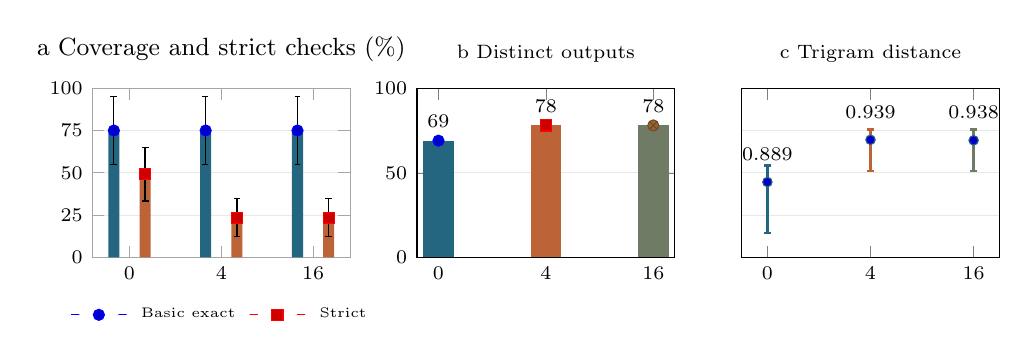
\begin{tikzpicture}
\pgfplotsset{every axis/.append style={every axis plot/.append style={mark=none},height=2.15cm,scale only axis,tick label style={font=\scriptsize},label style={font=\scriptsize},title style={font=\scriptsize},ymajorgrids=true,grid style={gray!18,line width=.3pt}}}
\begin{axis}[
  at={(0,0)},anchor=south west,width=0.27\textwidth,height=2.15cm,
  scale only axis,
  tick label style={font=\scriptsize},label style={font=\scriptsize},
  title style={font=\small,align=left},
  xtick={0,1,2},xticklabels={0,4,16},
  axis line style={gray!70,line width=.35pt},tick style={gray!70,line width=.35pt},
  ymajorgrids=true,grid style={gray!18,line width=.3pt},
  clip=false,
  title={a  Coverage and strict checks (\%)},
  ymin=0,ymax=100,ytick={0,25,50,75,100},
  legend style={at={(0.5,-0.23)},anchor=north,draw=none,font=\tiny,legend columns=2,column sep=3pt}
]
\addplot+[ybar,bar width=4pt,draw=none,fill=armzero] coordinates {(-0.17,75.00) (0.83,75.00) (1.83,75.00)};
\addplot+[ybar,bar width=4pt,draw=none,fill=armfour] coordinates {(0.17,49.17) (1.17,23.33) (2.17,23.33)};
\draw[black,line width=.45pt] (axis cs:-0.17,55.00) -- (axis cs:-0.17,95.00);
\draw[black,line width=.45pt] (axis cs:-0.21,55.00) -- (axis cs:-0.14,55.00);
\draw[black,line width=.45pt] (axis cs:-0.21,95.00) -- (axis cs:-0.14,95.00);
\draw[black,line width=.45pt] (axis cs:0.83,55.00) -- (axis cs:0.83,95.00);
\draw[black,line width=.45pt] (axis cs:0.79,55.00) -- (axis cs:0.86,55.00);
\draw[black,line width=.45pt] (axis cs:0.79,95.00) -- (axis cs:0.86,95.00);
\draw[black,line width=.45pt] (axis cs:1.83,55.00) -- (axis cs:1.83,95.00);
\draw[black,line width=.45pt] (axis cs:1.80,55.00) -- (axis cs:1.86,55.00);
\draw[black,line width=.45pt] (axis cs:1.80,95.00) -- (axis cs:1.86,95.00);
\draw[black,line width=.45pt] (axis cs:0.17,33.33) -- (axis cs:0.17,65.00);
\draw[black,line width=.45pt] (axis cs:0.14,33.33) -- (axis cs:0.21,33.33);
\draw[black,line width=.45pt] (axis cs:0.14,65.00) -- (axis cs:0.21,65.00);
\draw[black,line width=.45pt] (axis cs:1.17,12.50) -- (axis cs:1.17,35.00);
\draw[black,line width=.45pt] (axis cs:1.14,12.50) -- (axis cs:1.20,12.50);
\draw[black,line width=.45pt] (axis cs:1.14,35.00) -- (axis cs:1.20,35.00);
\draw[black,line width=.45pt] (axis cs:2.17,12.50) -- (axis cs:2.17,35.00);
\draw[black,line width=.45pt] (axis cs:2.13,12.50) -- (axis cs:2.21,12.50);
\draw[black,line width=.45pt] (axis cs:2.13,35.00) -- (axis cs:2.21,35.00);
\legend{Basic exact,Strict}
\end{axis}
\begin{axis}[at={(0.34\textwidth,0)},anchor=south west,width=0.27\textwidth,height=2.15cm,
  title={b  Distinct outputs},
  xtick={0,1,2},xticklabels={0,4,16},ymin=0,ymax=100,ytick={0,50,100}]
\addplot+[ybar,bar width=11pt,draw=none,fill=armzero] coordinates {(0,69)};
\addplot+[ybar,bar width=11pt,draw=none,fill=armfour] coordinates {(1,78)};
\addplot+[ybar,bar width=11pt,draw=none,fill=armsixteen] coordinates {(2,78)};
\node[font=\scriptsize,anchor=south] at (axis cs:0,71) {69};
\node[font=\scriptsize,anchor=south] at (axis cs:1,80) {78};
\node[font=\scriptsize,anchor=south] at (axis cs:2,80) {78};
\end{axis}
\begin{axis}[at={(0.68\textwidth,0)},anchor=south west,width=0.27\textwidth,height=2.15cm,
  title={c  Trigram distance},
  xtick={0,1,2},xticklabels={0,4,16},ymin=0.80,ymax=1.00,yticklabel=\empty,ytick style={draw=none},
  xmin=-0.25,xmax=2.25]
\addplot+[only marks,mark=*,mark size=1.7pt,color=armzero] coordinates {(0,0.88914) (1,0.93904) (2,0.9384)};
\draw[armzero,line width=1pt] (axis cs:0,0.82883) -- (axis cs:0,0.90897);
\draw[armzero,line width=1pt] (axis cs:-0.035,0.82883) -- (axis cs:0.035,0.82883);
\draw[armzero,line width=1pt] (axis cs:-0.035,0.90897) -- (axis cs:0.035,0.90897);
\draw[armfour,line width=1pt] (axis cs:1,0.9022) -- (axis cs:1,0.95086);
\draw[armfour,line width=1pt] (axis cs:0.965,0.9022) -- (axis cs:1.035,0.9022);
\draw[armfour,line width=1pt] (axis cs:0.965,0.95086) -- (axis cs:1.035,0.95086);
\draw[armsixteen,line width=1pt] (axis cs:2,0.90217) -- (axis cs:2,0.95096);
\draw[armsixteen,line width=1pt] (axis cs:1.965,0.90217) -- (axis cs:2.035,0.90217);
\draw[armsixteen,line width=1pt] (axis cs:1.965,0.95096) -- (axis cs:2.035,0.95096);
\node[font=\scriptsize,anchor=south] at (axis cs:0,0.90314) {0.889};\node[font=\scriptsize,anchor=south] at (axis cs:1,0.95304) {0.939};\node[font=\scriptsize,anchor=south] at (axis cs:2,0.9524) {0.938};
\end{axis}
\end{tikzpicture}
\caption{\textbf{Fragment penalties preserve exact coverage and increase lexical diversity, while fewer outputs pass strict structural checks.} Penalties 0, 4, and 16 each receive 120 tasks: 20 shared seeds, three length bands, and two search implementations. (a) Basic exact coverage is 90/120 in all conditions; strict selected-output coverage is 59/120, 28/120, and 28/120. (b) Distinct surface counts among the 90 successes. (c) Mean Jaccard distance between distinct texts' trigram sets; higher means less overlap. Lines in (a,c) are 95\% paired seed-bootstrap intervals. Distinct counts are finite-collection counts without bootstrap intervals.}
\label{fig:tradeoff}
\end{figure*}

\section{Paired intervention}
\paragraph{Search and admission.}
Both implementations start from empty text, using the same frozen vocabulary filtered from a 30K word list. Outside-in search extends outer word sequences toward their meeting point and closes when the unmatched character residual is itself a palindrome. Center-out search grows away from the center and closes on empty overhang. These closure rules differ; we compare penalties \emph{within} each method, without attributing differences to direction alone.

The baseline score adds English Zipf word frequency \citep{speer-2022-wordfreq} and 0.3 per character, subtracts 2 per prior use of a word and 4 for adjacent repetition, and adds seeded perturbations for beam ranking. Selection uses the unperturbed accumulated score per normalized letter. The shared basic gate requires ASCII rendering, exact normalized-letter reversal, the requested length band, lexicon membership, a fixed allowlist for words of at most two letters, and exclusions for listed catalogue examples and templates. Repeated words are permitted.

A stricter post-selection screen also rejects self-palindromic words and proper multiword spans, repeated multiword units, whole-word reversals, and other mechanical shortcuts. It neither reruns search nor measures grammaticality. We report both basic and strict coverage over \emph{all requested tasks}.

\paragraph{Frozen penalty.}
We select the six most prevalent word trigrams from the prior 52 distinct texts, breaking ties alphabetically: \emph{no it a}, \emph{a i cos}, \emph{it a i}, \emph{cos same open}, \emph{i cos same}, and \emph{one poem association}. Each prior text contributes at most one prevalence vote per trigram. The new search does not update this list.

Let $F(x)$ count occurrences of these trigrams in the current concatenated word sequence, including overlaps. For a parent state $x$ and child $x'$, we replace the baseline score increment $\Delta S$ with
\begin{equation}
\Delta S_\lambda=\Delta S-\lambda\bigl[F(x')-F(x)\bigr].
\end{equation}
The changes telescope to a final charge $-\lambda F(x)$. This matters when outside-in growth breaks a temporary join: its penalty is refunded. We test $\lambda\in\{0,4,16\}$, fixed before new outputs or ratings were inspected. The penalty affects beam ranking and final selection; vocabulary and admission gates remain identical.

\paragraph{Matched tasks and resources.}
The experiment crosses 20 fresh seeds (7100--7119), three normalized-letter bands (30--49, 50--79, 80--119), both methods, and three penalty levels: 360 jobs. Each seed--band--method block runs all penalties sequentially on one worker, in seeded random order. All receive beam width 256, candidate limit 800, per-parent limit 32, at most 400 steps, 32 words, 24 residual letters, and a 180-second cooperative wall budget. Thirty-two workers run on one AWS c7i.16xlarge CPU instance. No job reaches its deadline; mean run times are 2.96, 3.04, and 3.03 seconds. Equal limits need not imply equal expansions, so scorer-call counts are retained.

\section{Measurements}
\paragraph{Coverage and diversity.}
Coverage includes failures in the denominator. Lexical analyses collapse identical surfaces within each arm and tokenize lowercase ASCII words. For trigram sets $A$ and $B$, distance is $1-|A\cap B|/|A\cup B|$; we average across every unordered pair of distinct texts. We also report the maximum prevalence of \emph{any} trigram, targeted-fragment prevalence, and distinct surface counts. Measuring all trigrams can expose replacement repetition that a targeted-fragment count misses.

\begin{figure*}[t]
\centering
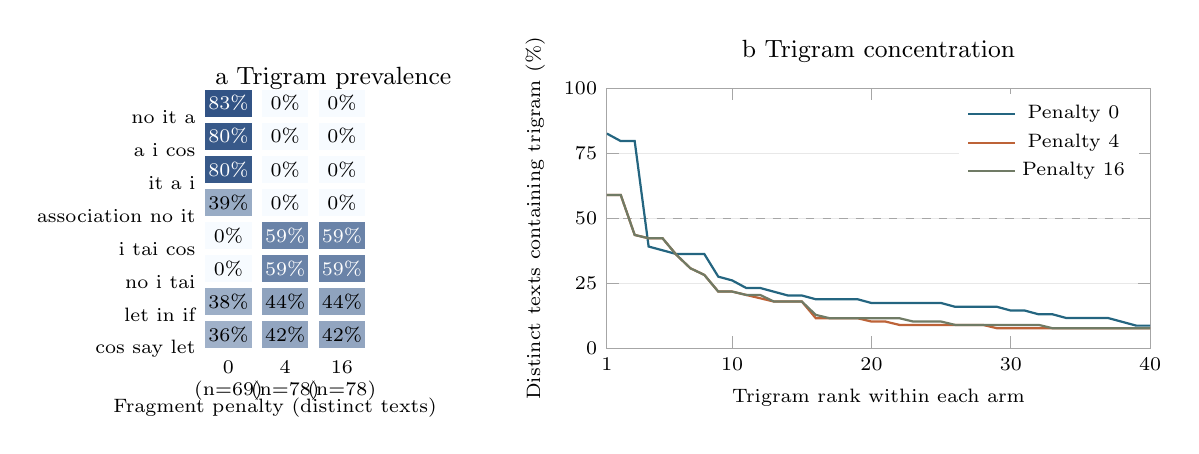
\begin{tikzpicture}[x=0.72cm,y=0.42cm]
\begin{scope}
  \node[anchor=west,font=\small] at (0,8.15) {a  Trigram prevalence};
  \node[anchor=east,font=\scriptsize] at (0,7) {no it a};\node[anchor=east,font=\scriptsize] at (0,6) {a i cos};\node[anchor=east,font=\scriptsize] at (0,5) {it a i};\node[anchor=east,font=\scriptsize] at (0,4) {association no it};\node[anchor=east,font=\scriptsize] at (0,3) {i tai cos};\node[anchor=east,font=\scriptsize] at (0,2) {no i tai};\node[anchor=east,font=\scriptsize] at (0,1) {let in if};\node[anchor=east,font=\scriptsize] at (0,0) {cos say let};
  \definecolor{motif1}{HTML}{325385}\fill[motif1] (0,7) rectangle ++(0.82,0.82);\node[font=\scriptsize,text=white] at (0.41,7.41) {83\%};\definecolor{motif2}{HTML}{F7FBFF}\fill[motif2] (1,7) rectangle ++(0.82,0.82);\node[font=\scriptsize,text=black] at (1.41,7.41) {0\%};\definecolor{motif3}{HTML}{F7FBFF}\fill[motif3] (2,7) rectangle ++(0.82,0.82);\node[font=\scriptsize,text=black] at (2.41,7.41) {0\%};\definecolor{motif4}{HTML}{385989}\fill[motif4] (0,6) rectangle ++(0.82,0.82);\node[font=\scriptsize,text=white] at (0.41,6.41) {80\%};\definecolor{motif5}{HTML}{F7FBFF}\fill[motif5] (1,6) rectangle ++(0.82,0.82);\node[font=\scriptsize,text=black] at (1.41,6.41) {0\%};\definecolor{motif6}{HTML}{F7FBFF}\fill[motif6] (2,6) rectangle ++(0.82,0.82);\node[font=\scriptsize,text=black] at (2.41,6.41) {0\%};\definecolor{motif7}{HTML}{385989}\fill[motif7] (0,5) rectangle ++(0.82,0.82);\node[font=\scriptsize,text=white] at (0.41,5.41) {80\%};\definecolor{motif8}{HTML}{F7FBFF}\fill[motif8] (1,5) rectangle ++(0.82,0.82);\node[font=\scriptsize,text=black] at (1.41,5.41) {0\%};\definecolor{motif9}{HTML}{F7FBFF}\fill[motif9] (2,5) rectangle ++(0.82,0.82);\node[font=\scriptsize,text=black] at (2.41,5.41) {0\%};\definecolor{motif10}{HTML}{99ACC5}\fill[motif10] (0,4) rectangle ++(0.82,0.82);\node[font=\scriptsize,text=black] at (0.41,4.41) {39\%};\definecolor{motif11}{HTML}{F7FBFF}\fill[motif11] (1,4) rectangle ++(0.82,0.82);\node[font=\scriptsize,text=black] at (1.41,4.41) {0\%};\definecolor{motif12}{HTML}{F7FBFF}\fill[motif12] (2,4) rectangle ++(0.82,0.82);\node[font=\scriptsize,text=black] at (2.41,4.41) {0\%};\definecolor{motif13}{HTML}{F7FBFF}\fill[motif13] (0,3) rectangle ++(0.82,0.82);\node[font=\scriptsize,text=black] at (0.41,3.41) {0\%};\definecolor{motif14}{HTML}{6A83A8}\fill[motif14] (1,3) rectangle ++(0.82,0.82);\node[font=\scriptsize,text=white] at (1.41,3.41) {59\%};\definecolor{motif15}{HTML}{6A83A8}\fill[motif15] (2,3) rectangle ++(0.82,0.82);\node[font=\scriptsize,text=white] at (2.41,3.41) {59\%};\definecolor{motif16}{HTML}{F7FBFF}\fill[motif16] (0,2) rectangle ++(0.82,0.82);\node[font=\scriptsize,text=black] at (0.41,2.41) {0\%};\definecolor{motif17}{HTML}{6A83A8}\fill[motif17] (1,2) rectangle ++(0.82,0.82);\node[font=\scriptsize,text=white] at (1.41,2.41) {59\%};\definecolor{motif18}{HTML}{6A83A8}\fill[motif18] (2,2) rectangle ++(0.82,0.82);\node[font=\scriptsize,text=white] at (2.41,2.41) {59\%};\definecolor{motif19}{HTML}{9DAFC7}\fill[motif19] (0,1) rectangle ++(0.82,0.82);\node[font=\scriptsize,text=black] at (0.41,1.41) {38\%};\definecolor{motif20}{HTML}{8FA3BE}\fill[motif20] (1,1) rectangle ++(0.82,0.82);\node[font=\scriptsize,text=black] at (1.41,1.41) {44\%};\definecolor{motif21}{HTML}{8FA3BE}\fill[motif21] (2,1) rectangle ++(0.82,0.82);\node[font=\scriptsize,text=black] at (2.41,1.41) {44\%};\definecolor{motif22}{HTML}{A0B1C9}\fill[motif22] (0,0) rectangle ++(0.82,0.82);\node[font=\scriptsize,text=black] at (0.41,0.41) {36\%};\definecolor{motif23}{HTML}{92A5C0}\fill[motif23] (1,0) rectangle ++(0.82,0.82);\node[font=\scriptsize,text=black] at (1.41,0.41) {42\%};\definecolor{motif24}{HTML}{92A5C0}\fill[motif24] (2,0) rectangle ++(0.82,0.82);\node[font=\scriptsize,text=black] at (2.41,0.41) {42\%};
  \node[font=\scriptsize,anchor=north,align=center] at (0.41,-0.08) {0\\(n=69)};\node[font=\scriptsize,anchor=north,align=center] at (1.41,-0.08) {4\\(n=78)};\node[font=\scriptsize,anchor=north,align=center] at (2.41,-0.08) {16\\(n=78)};
  \node[font=\scriptsize,anchor=north] at (1.23,-1.2) {Fragment penalty (distinct texts)};
\end{scope}
\begin{scope}[xshift=5.1cm]
  \begin{axis}[
    at={(0,0)},anchor=south west,width=6.9cm,height=3.3cm,scale only axis,
    title={b  Trigram concentration},title style={font=\small,align=left},
    xlabel={Trigram rank within each arm},ylabel={Distinct texts containing trigram (\%)},
    xmin=1,xmax=40,ymin=0,ymax=100,xtick={1,10,20,30,40},ytick={0,25,50,75,100},
    tick label style={font=\scriptsize},label style={font=\scriptsize},
    axis line style={gray!70,line width=.35pt},tick style={gray!70,line width=.35pt},
    ymajorgrids=true,grid style={gray!18,line width=.3pt},
    legend style={draw=none,font=\scriptsize,at={(0.98,0.98)},anchor=north east}
  ]
\addplot[gray!70,dashed,line width=.4pt,forget plot] coordinates {(1,50)(40,50)};
  \addplot+[no marks,line width=.8pt,color=armzero] coordinates {(1,82.609) (2,79.710) (3,79.710) (4,39.130) (5,37.681) (6,36.232) (7,36.232) (8,36.232) (9,27.536) (10,26.087) (11,23.188) (12,23.188) (13,21.739) (14,20.290) (15,20.290) (16,18.841) (17,18.841) (18,18.841) (19,18.841) (20,17.391) (21,17.391) (22,17.391) (23,17.391) (24,17.391) (25,17.391) (26,15.942) (27,15.942) (28,15.942) (29,15.942) (30,14.493) (31,14.493) (32,13.043) (33,13.043) (34,11.594) (35,11.594) (36,11.594) (37,11.594) (38,10.145) (39,8.696) (40,8.696)};\addplot+[no marks,line width=.8pt,color=armfour] coordinates {(1,58.974) (2,58.974) (3,43.590) (4,42.308) (5,42.308) (6,35.897) (7,30.769) (8,28.205) (9,21.795) (10,21.795) (11,20.513) (12,19.231) (13,17.949) (14,17.949) (15,17.949) (16,11.538) (17,11.538) (18,11.538) (19,11.538) (20,10.256) (21,10.256) (22,8.974) (23,8.974) (24,8.974) (25,8.974) (26,8.974) (27,8.974) (28,8.974) (29,7.692) (30,7.692) (31,7.692) (32,7.692) (33,7.692) (34,7.692) (35,7.692) (36,7.692) (37,7.692) (38,7.692) (39,7.692) (40,7.692)};\addplot+[no marks,line width=.8pt,color=armsixteen] coordinates {(1,58.974) (2,58.974) (3,43.590) (4,42.308) (5,42.308) (6,35.897) (7,30.769) (8,28.205) (9,21.795) (10,21.795) (11,20.513) (12,20.513) (13,17.949) (14,17.949) (15,17.949) (16,12.821) (17,11.538) (18,11.538) (19,11.538) (20,11.538) (21,11.538) (22,11.538) (23,10.256) (24,10.256) (25,10.256) (26,8.974) (27,8.974) (28,8.974) (29,8.974) (30,8.974) (31,8.974) (32,8.974) (33,7.692) (34,7.692) (35,7.692) (36,7.692) (37,7.692) (38,7.692) (39,7.692) (40,7.692)};
  \legend{Penalty 0,Penalty 4,Penalty 16}
  \end{axis}
\end{scope}
\end{tikzpicture}
\caption{\textbf{Removing named fragments leaves new concentrations.} (a) The union of the four most prevalent trigrams at penalties 0 and 4, ordered by descending count with alphabetical tie-breaking within each condition. Each cell is the fraction of distinct texts containing that trigram; overlapping trigrams are counted separately. (b) Prevalence of the 40 highest-ranked trigrams in each arm. The leading concentration falls from 57/69 (82.6\%) to 46/78 (59.0\%), but a majority still share a trigram. All six targeted trigrams are absent from both penalized arms, including targets outside the displayed rows.}
\label{fig:motifs}
\end{figure*}

\paragraph{Seed-level uncertainty.}
We use 20,000 paired percentile bootstrap replicates, resampling the 20 seeds and retaining their methods, bands, and arms together (PRNG seed 20261002). Conditional diversity is recomputed after collapsing duplicate surfaces in each resample. These intervals describe search-seed variability on this vocabulary, not independent semantic tasks. Pairwise text comparisons are not treated as independent trials. We report both strengths against baseline without selecting a winning strength or computing confirmatory $p$-values. Raw distinct counts receive no bootstrap interval because resampling observed strings biases richness downward.

\paragraph{Blinded model audit.}
A separate Qwen3 32B audit on AWS Bedrock \citep{awsbedrockqwen332b} uses the existing 0--3 grammaticality and coherent-meaning rubric. The model sees one exact text, with no method or penalty label. A joint pass requires at least 2 on both scales. The control gate requires at least 8/12 held-out Brown prose controls \citep{kucera-francis-1967} and at most 3/12 corresponding shuffles to pass. All 148 distinct new texts are rated once; shared texts receive the same rating across arms. Twelve hidden repeats test consistency. Appendix~\ref{sec:rubric} specifies the protocol. The control gate tests coarse prose detection, not palindrome-domain calibration. These are model ratings, without human validation.

\section{Results}
\paragraph{Exact yield is unchanged.}
Every penalty returns 90 basic-valid outputs from 120 requested tasks, with 15/20 successes in each method--band cell. Success and failure occur on the same paired tasks. The observed paired yield differences and their bootstrap intervals are zero; this does not establish population equivalence.

\paragraph{Lexical diversity increases.}
At $\lambda=4$, distinct texts increase from 69 to 78 and mean pairwise trigram distance rises from 0.889 to 0.939 (difference $+0.050$, 95\% paired interval $[0.026,0.087]$). Maximum trigram prevalence falls from 82.6\% to 59.0\% (difference $-23.6$ percentage points, interval $[-37.2,-7.9]$). The $\lambda=16$ arm has 78 distinct texts, distance 0.938, and the same maximum prevalence. Its selected text differs from $\lambda=4$ on eight tasks. Figure~\ref{fig:tradeoff} reports the full comparison.

\paragraph{Repetition changes form.}
Both penalties remove all six targeted trigrams from all 90 selected outputs. Nevertheless, \emph{i tai cos} and \emph{no i tai} each appear in 46/78 distinct texts. Figure~\ref{fig:motifs} shows both their prevalence and the broader recurrence distribution. A zero count for the targeted list would conceal this concentration.

\paragraph{Structural shortcuts increase.}
Strict coverage decreases from 59/120 to 28/120 for both penalties: $-25.8$ percentage points, paired interval $[-37.5,-15.0]$. Proper self-palindromic multiword spans fail the strict check in 58/90 outputs at $\lambda=4$ and 61/90 at $\lambda=16$; self-palindromic words fail in 16/90 under each. These overlapping failure counts describe structural properties, not sentence quality.

\paragraph{Language-quality check.}
Qwen3 passes 11/12 prose controls and 0/12 shuffles. None of the 148 distinct candidates reaches the joint threshold: 142 receive $(0,0)$, three $(1,0)$, and three $(1,1)$ for grammar and meaning. All 12 hidden repeats agree exactly. The penalties therefore provide no threshold-passing candidate under this rubric; these near-floor ratings do not establish equivalence or human unreadability.

\section{Discussion and conclusion}
The intervention changes the intended lexical metrics: targeted fragments disappear, overlap decreases, and surface variety increases at the same exact-output yield. It also shifts repetition toward other fragments and selects more outputs rejected by a separate structural screen. The tradeoff would be missed by reporting only exactness and avoidance of a fixed list.

For this search family, fragment penalties warrant evaluation against untargeted recurrence and structural admission as well as their own objective. A human study with explicit dimensions and quality checks \citep{khashabi-etal-2022-genie} remains necessary for a reader-quality claim. The experiment provides a controlled comparison within two implementations, rather than a benchmark advantage over published generators.

\paragraph{Reproducibility.}
The supplement contains the frozen protocol, vocabulary, 360 job records, scorer implementation, raw model responses, analysis, and figure source. Input and source hashes are checked before search. The offline analysis reproduces both figures and the paired intervals without new inference. AWS resources were private and temporary; Brown corpus text is omitted from the release.

\section*{Limitations}
The intervention was motivated by an inspected historical collection; its six targets and two strengths are not a general diversity objective. Fresh seeds separate development observations from these jobs, but all share one vocabulary and search implementation family. The methods' native closure rules differ. Diversity conditions on successful outputs, and duplicate collapse does not remove shared-fragment dependence. Seed-bootstrap intervals do not measure uncertainty over languages, semantic tasks, or readers; deduplicated diversity is a nonlinear statistic with a small number of clusters. The strict screen is mechanical and may reject readable palindromes. Qwen's small control screen has no human calibration, and possible pretraining exposure to Brown is unknown. Hosted inference has no provider seed or exposed weight digest. There are no human ratings or matched external-generator results.

\section*{Ethical considerations}
No participant data were collected. Model ratings must not be presented as human judgments. Generative AI assisted implementation, writing, and internal review.

\bibliography{refs}
\appendix
\section{Search implementation and execution}
The baseline uses \code{wordfreq} 3.1.1. A seeded uniform perturbation in $[0,0.4)$ is added to child priorities for exploration and excluded from the accumulated score used for closure selection. The fragment penalty is computed as an exact potential difference, including current left--right joins. Exhaustive toy tests over both growth directions verify local increments against full-sequence recounting and verify that broken joins are refunded. At zero strength the wrapper returns the baseline score unchanged.

All 360 jobs completed without execution errors or deadline exits. The search instance used 32 workers on 64 virtual CPUs. Mean scorer-call counts were 56,415, 52,679, and 52,722 for penalties 0, 4, and 16. These counts describe evaluated word extensions, not language-model calls. Both gates, every failed job, and elapsed times are retained. The strict screen is applied to the selected basic-valid output; search is not repeated when that output fails it.

\section{Model rubric and controls}\label{sec:rubric}
The model is \code{qwen.qwen3-32b-v1:0} on Bedrock in \code{us-east-2}, using temperature 0, top-p 1, maximum 128 output tokens, a no-thinking directive, and a structured JSON response. The prompt asks the judge to assess the exact text without repair or rewards for symmetry.

Grammar anchors are: 0, no recoverable sentence parse; 1, isolated grammatical phrases with major sentence breaks; 2, a mostly recoverable but strained parse; 3, natural grammatical connected English. Meaning anchors are: 0, no recoverable proposition or event; 1, word associations with unclear relations; 2, a plausible but incomplete or vague interpretation; 3, clear meaning with understandable relations.

The 12 prose and 12 shuffle controls are the same hash-verified Brown spans used in the prior audit; seven prose controls contain multiple sentences. After the control gate, 148 distinct candidates and 12 repeats are presented in a fixed hash-derived order. Repeats comprise six candidates and six prose controls selected by ascending text hash. The full presentation inventory was fixed after generation and before new judge calls; the rubric and decision thresholds predate generation. Only the exact text and rubric enter model messages. Ratings do not influence generation or selection.

\section{Historical development collection}
The six targets come from 52 distinct texts among 66 outputs in an earlier 240-job resource comparison. In that collection, Brown and GPT-2 shuffle-relative contrasts disagree in sign for 28/52 texts, and 63/66 GPT-2 originals lie inside their 32-shuffle score ranges. Those descriptive findings motivate separate diagnostics but do not serve as inferential evidence for this intervention. The prior outputs, diagnostics, and figure builder remain in the supplement. The new experiment uses disjoint seeds and compares penalties at one fixed resource configuration.

\section{Exploratory long-output probe}
A separate development probe used two seeds, both search implementations, letter bands 120--159 and 800--999, and word caps 32 and 256 (16 jobs). With cap 256, two of four long-band jobs returned exact 804-letter, 184-word outputs; neither passed the strict screen. The two outputs share a word multiset and have no readability ratings. The longest vocabulary word has 18 letters, so cap 32 cannot exceed 576 letters. This bound was noticed after execution: the infeasible arm is not a performance baseline. An interrupted execution retained four checkpoints and restarted the remaining twelve jobs; uncheckpointed outcomes are unknown. The supplement retains the protocol, all recorded outcomes, renderings, and an independent reversal verifier. These exploratory results are separate from the 360-job intervention.

\section{Offline reproduction}
Install \path{paper/figure-requirements.txt} and run \path{experiments/analyze_fragment_penalty_20261002.py} from the supplement root. It verifies protocol and text hashes, recomputes endpoints and intervals, and rebuilds figures. The archived responses support the model audit. Offline analysis needs no corpus download, model weights, or AWS account.
\end{document}
